%test
\documentclass[ngerman,
a4paper,     %% defines the paper size: a4paper (default), a5paper, letterpaper, ...
% landscape,   %% sets the orientation to landscape
oneside,     %% changes to a two-page-layout (alternatively: oneside)
%autooneside,
% twocolumn,   %% changes to a two-column-layout
 %headsepline, %% add a horizontal line below the column title
 %footsepline, %% add a horizontal line above the page footer
% titlepage,   %% only the titlepage (using titlepage-environment) appears on the first page (alternatively: notitlepage)
parskip,     %% insert an empty line between two paragraphs (alternatively: halfparskip, ...)
% leqno,       %% equation numbers left (instead of right)
 fleqn,       %% equation left-justified (instead of centered)
% tablecaptionabove, %% captions of tables are above the tables (alternatively: tablecaptionbelow)
% draft,       %% produce only a draft version (mark lines that need manual edition and don't show graphics)
bibliography=totoc,index=totoc,listof=totoc, %Literaturverzeichnis usw auch in die Inhaltsangabe
% 10pt,       %% set default font size to 10 point 
 12pt,         %% set default font size to 11 point
%11pt         %% set default font size to 12 point
 DIV=10, 
 BCOR=10mm,
]{scrreprt}  %% article, see KOMA documentation (scrguide.dvi) 

% Für oft geforderte 1,5 Zeilenhöhe
\usepackage{setspace}
\onehalfspacing 

%\KOMAoption{fontsize=14pt}

% natbib für deutsche Zitate
%\usepackage[numbers,sort&compress,super]{natbib}
\usepackage[]{natbib} 

\usepackage{import} 

%\usepackage[american]{babel}
\usepackage[ngerman]{babel}
\usepackage{blindtext}

%%% inputenc: coding of german special characters
\usepackage[utf8]{inputenc}

%%% fontenc, ae, aecompl: coding of characters in PDF documents
\usepackage[T1]{fontenc}
%\usepackage{ae,aecompl}
\usepackage{lmodern}

\makeatletter
\newcommand\cellwidth{\TX@col@width}
\makeatother

% source Code darstellen
\usepackage[formats]{listings}
\lstdefineformat{Java}
{
	\{=\newline\string\newline\indent,%
	\}=\newline\noindent\string\newline,%
	;=[\ ]\string\space,%
}
\usepackage{color}
\definecolor{javared}{rgb}{0.6,0,0} % for strings
\definecolor{javagreen}{rgb}{0.25,0.5,0.35} % comments
\definecolor{javapurple}{rgb}{0.5,0,0.35} % keywords
\definecolor{javadocblue}{rgb}{0.25,0.35,0.75} % javadoc

\lstset{language=Java,
	format=Java,
	basicstyle=\ttfamily,
	keywordstyle=\color{javapurple}\bfseries,
	stringstyle=\color{javared},
	commentstyle=\color{javagreen},
	morecomment=[s][\color{javadocblue}]{/**}{*/},
	numbers=left,
	numberstyle=\tiny\color{black},
	stepnumber=1,
	numbersep=10pt,
	tabsize=4,
	showspaces=false,
	showstringspaces=false,
	breaklines=true,
	breakatwhitespace=true,
	frame=single,
	}
	
%Copyrights 
% graphicx mus bei Verwendung auskommentiert werden
% ohne textcomp gab es warning 
\usepackage{textcomp}
\usepackage{caption, copyrightbox} 
% Schriftart für copyrights ändern, da es sonst Warnung 
% gab wegen deprecated Schriftart
\makeatletter 
\renewcommand{\CRB@setcopyrightfont}{%
\footnotesize
\color{gray!70}
\usefont{T1}{phv}{m}{n}
}
\makeatother

\usepackage{tabularx}
\usepackage{longtable}

\usepackage{units} 

\makeatletter
    \@ifpackageloaded{tex4ht}{
      \usepackage[dvips]{color,graphicx}
      \usepackage[tex4ht,colorlinks,allcolors = black]{hyperref}
	}
	{ 
      \usepackage[colorlinks,allcolors = black]{hyperref}
	}
\makeatother 

%\usepackage{pdfpages}

\usepackage{enumitem} %For list environments
\setlist{itemsep=-1em,topsep=-1em}


\usepackage[babel=true,strict=true,german=quotes,threshold=1]{csquotes}


% \publishers{}

% \thanks{} %% use it instead of footnotes (only on titlepage)

% \dedication{} %% generates a dedication-page after titlepage


\usepackage{amsmath}
\numberwithin{equation}{section}

\usepackage{scrpage2}

\usepackage[noabbrev]{cleveref}

%%% scrheadings default: 
%%%      footer - middle: page number
\pagestyle{scrheadings}

%\pagestyle{empty} % Seiten ohne Header
%
% loescht voreingestellte Stile
\clearscrheadfoot
 
%
% Was steht wo...
   %\ohead{\headmark - \pagemark}
   %\ihead{\headmark}

\title{GeoQuest}

\begin{document}

\subject{Diplomarbeit}   %% subject which
% appears above titlehead

\subtitle{Bewegung durch Technik}

%%% author(s)
%\author{Yasmin Musterfrau \and Max Mustermann \and Author DerDritte}

%%% date
\date{Imst, \today} 

\titlehead{
\begin{minipage}[b]{0.64\textwidth}
%\vspace{-30mm}
%\hspace{-4mm}

\includegraphics[height=3.5cm]{GeoQuest} % logo
\end{minipage}
\begin{minipage}[b]{0.35\textwidth}
%\vspace{-32mm}
\begin{flushright}

\includegraphics[height=3cm]{Logo_HAK_Imst} % logo
\end{flushright}
\end{minipage}
%\\
%\centerline{\hrulefill}
}%end of titlehead
%\titlehead{Tierphysiologische Übungen Teil Dr. Hans Moser 
%\vspace{5mm}
%\includegraphics*{Bilder/UniLogo} % kleines logo
%}




\publishers{
\footnotesize
Eingereicht von 

\begin{tabular}{ l c r }
  Christopher Haider & Verantwortlich für IT: HTML, CSS, BWL: Kaufvertrag \\
  Maximilian Egger & Verantwortlich für IT: HTML, CSS, BWL: Kaufvertrag \\
  Dominik Neuner & Verantwortlich für Kontrolle\\
  \\\\
\end{tabular}

Eingereicht bei \\
Alexander Scharmer, Claudio Landerer und Stefan Stolz
}

\def \currentAuthor {}

\makeatletter
\let\newtitle\@title
\let\newauthor\@author
\let\newdate\@date
\makeatother

%Muss in der Reihenfolge stehen!:
\automark[subsection]{section}
%\ohead{\pagemark}
\ihead{\newtitle}
%\lehead{\rightmark}
%\lohead{\leftmark}
%\lefoot{Ausgearbeitet von \ldots}
%\refoot{Skriptum Thermodynamik}
\rofoot{Seite \thepage{}}
\lofoot{Verantwortlich für den Inhalt: \currentAuthor}

\newcaptionname{ngerman}{\lstlistlistingname}{Quelltexte} %Table of listings 
\newcaptionname{ngerman}{\lstlistingname}{Quelltext}      %Listing
\lstMakeShortInline[columns=fixed]|
 
\maketitle

\chapter*{Eidesstattliche Erklärung}
Ich erkläre an Eides statt, dass ich die vorliegende Diplomarbeit selbst verfasst und keine anderen als die angeführten Behelfe verwendet habe. Alle Stellen, die wörtlich oder inhaltlich den angegebenen Quellen entnommen wurden, sind als solche kenntlich gemacht.
Ich bin damit einverstanden, dass meine Arbeit öffentlich zugänglich gemacht wird.

\vspace{1cm}
\begin{tabular}{c c c}
	& \hspace{4cm} & \\\cline{1-1}
	Ort, Datum & & \\
	\vspace{2cm}
	& & \\\cline{1-1}\cline{3-3}
	Christopher Haider & & Maximilian Egger \\ 
	\vspace{2cm}
	& & \\\cline{1-1}\cline{3-3}
	Dominik Neuner & & Harald Sommer \\ 
\end{tabular}

\chapter*{Abnahmeerklärung}
Hiermit bestätigt der Auftraggeber, dass das übergebene Produkt dieser Diplomarbeit den dokumentierten Vorgaben entspricht. Des Weiteren verzichtet der Auftraggeber auf unentgeltliche Wartung und Weiterentwicklung des Produktes durch die Projektmitglieder bzw. die Schule.

\vspace{1cm}
\begin{tabular}{c}
	\\\cline{1-1}
	Ort, Datum\\
	\vspace{2cm}
	\\\cline{1-1}
	Auftraggeber
\end{tabular}	

\chapter*{Vorwort}
z. B. Hinweise, wie das bearbeitete Thema gefunden wurde oder Dank für die Betreuung (Kooperationspartner/in, Betreuer/innen, Sponsoren) etc.


\chapter*{Abstract (Deutsch)}
Es soll eine Applikation entwickelt werden, bei der Fragen (zu einem Thema) und zugehörigen mögliche Antworten (mit einer richtigen) erstellt werden können. Jeder Frage muss ein Standort auf der Karte zugewiesen werden. 
Im Front-End können Fragen im Umkreis aufgelistet und gelöst werden. Für jede gelöste Frage erhöht sich der Punktestand des Benutzers.  


\chapter*{Abstract (Englisch)}
An App should  be developed, where questions (to a topic) and the belonging answers (with one correct)  are able to be created. Each Question must have a location on the map. In the front-end-mode questions in permiter can be listed and solved. After every solved Question the score of the user will be increased.

\tableofcontents 

\def \currentAuthor {Gabi Sorglos} %so kann jederzeit der Autor geändert werden -> wird in der Fusszeile angezeigt.

\chapter*{Einleitende Bemerkungen}

\chapter*{Notationen}
Beschreibung wie Code, Hinweise, Zitate etc. formatiert werden  

\chapter{Projektmanagement}

\section{Metainformationen}
\subsection{Team}
Christopher Haider (Leiter, Programmierer, Design)\begin{figure}
	\centering
	\includegraphics[width=0.4\linewidth]{C:/Users/Christopher/Downloads/2ITA_Haider_Christopher}
	\caption{}
	\label{fig:2itahaiderchristopher}
\end{figure}

Maximilian Egger (Programmierer, Druck)\begin{figure}
	\centering
	\includegraphics[width=0.4\linewidth]{C:/Users/Christopher/Downloads/MAxi}
	\caption{}
	\label{fig:maxi}
\end{figure}

\subsection{Betreuer}
NEUNER Dominik, MSc
\subsection{Partner}
HAK Imst
\subsection{Ansprechpartner}
NEUNER Dominik, MSc
\section{Vorerhebungen}
\subsection{Projektzieleplan}

\textbf {-Einteilung:}


\textbf {OBERZIEL} Es soll eine Applikation entwickelt werden, bei der Fragen (zu einem Thema) und zugehörigen mögliche Antworten (mit einer richtigen) erstellt werden können. Jeder Frage muss ein Standort auf der Karte zugewiesen werden.
Im Front-End können Fragen im Umkreis aufgelistet und gelöst werden. Für jede gelöste Frage erhöht sich der Punktestand des Benutzers.  


\textbf {LEISTUNGSZIEL} Das Projekt wird mehrere Mitarbeiter beinhalten und wir versuchen den einzelnen Mitarbeitern die optimale Arbeit zuzuweisen, um eine pünktliche Fertigstellung mit würdiger Qualität zu erreichen. Implementierung von aktuellen Karten und Standort, kleine Übersicht des Punktestandes, Backend/Frontend;


\textbf {KOSTENZIEL} Die Kosten belaufen sich ca. in Höhe von 8.500 - 12.500 € abhängig von der Zeit der aktiven Arbeit jedes einzelnen Mitarbeiters/Programmierer plus den Überstunden inklusive allen Aufwänden für die Programmierung, Serverwartungen, laufende Aktualisierungen von den Daten. Abgesehen von den Steuern.


\textbf {TERMINZIEL} Dieses etwas umfangreichere Projekt sollte mit Einplanung vom 14.03.2017 in einem Zeitrahmen bis Ende November/Dezember in Form von einer kompakten App im Store verfügbar sein.


\textbf {DETAILZIEL} Unserem Partner/Kunden vor der endgültigen Fertigstellung des Projekts eine Testapp /  Prototypapp vorzeigen und nochmals eine endgültige Absprache mit den Kunden abhalten.



\subsection{Projektumfeld}

\begin{figure}
	\centering
	\includegraphics[width=1\linewidth]{../Grafik1}
	\caption{Projektnähe tabellarisch}
	\label{fig:grafik1}
\end{figure}


\begin{figure}
	\centering
	\includegraphics[width=1\linewidth]{../Grafik}
	\caption{Projektnähe Grafisch}
	\label{fig:grafik}
\end{figure}




Welche Bedrohungen bestehen für das Projekt
Budget Überschreitung
\begin{itemize}
	\item Termine nicht einhalten
	\item Auftragsgeber sagt ab
	\item Auftragsgeber ändert seine Anforderungen
	\item Probleme bei der Realisierung
\end{itemize}



\subsection{Risikoanalyse}
\begin{figure}
	\centering
	\includegraphics[width=1.2\linewidth]{../Grafik2}
	\caption{Risikomatrix}
	\label{fig:grafik2}
\end{figure}

\section{Pflichtenheft}
\subsection{Zielbestimmung}

\textbf {Projektbeschreibung}
 Es soll eine Applikation entwickelt werden, bei der Fragen (zu einem Thema) und zugehörigen mögliche Antworten (mit einer richtigen) erstellt werden können. Jeder Frage muss ein Standort auf der Karte zugewiesen werden.
Im Front-End können Fragen im Umkreis aufgelistet und gelöst werden. Für jede gelöste Frage erhöht sich der Punktestand des Benutzers.

\textbf {IST-Zustand}
Diese Applikation gibt es nach dieser Weise noch nicht, dennoch sind Ähnlichkeiten mit Pokemon Go zu erkennen. Obwohl es nicht um Pokemon geht, sonder um Fragen und Antworten die einen Standort besitzen.

\textbf {SOLL-Zustand}
Diese Applikation soll dem Nutzer die Möglichkeit geben Informatik außerhalb des Gebäudes zu beantworten. Dies soll die Anwender anregen mehr ins freie zu gehen um Sport zu betreiben, dennoch sein Wissen im Bereich IT zu erweitern


\subsection{Produkteinsatz und Umgebung}
\begin{itemize}
	\item in Form einer App im Store erhältlich
	\item Jugendliche und Erwachsene
	\item Lizenz
	\item GPS, Android-Phone und Internetverbindung
\end{itemize}
\subsection{Funktionalitäten}
\begin{itemize}
	\item MUSS-Anforderungen

		
		Funktionale Anforderung
		\item Fragen hinzufügen, Antworten hinzufügen, Punktestand erhöhen, Standort muss sich ändern können, Absturz der App vermeiden
		
		Nicht Funktionale Anforderung
		\item auf allen Plattformen erhältlich,Man muss Designs bearbeiten, Kein Widerspruch gegenüber Kunde und dem Team, welches den Auftrag erfüllen soll
		
	
	\item KANN-Anforderungen
	
		
		Funktionale Anforderung
		\item Man kann noch weiter Backupfunktionen miteinbeziehen (Serverbezogen)
		
		Nicht Funktionale Anforderung
		\item Kann als App und Webseite verwendet werden 
		

\end{itemize}
\subsection{Testszenarien und Testfälle}
\begin{itemize}
	\item Beschreibung der Testmethodik
	\item Testfall 1
	\item Testfall 2
	\item \ldots
\end{itemize}
\subsection{Liefervereinbarung}
\begin{itemize}
	\item Applikation
	\item Adminmodus, Benutzermodus
	\item Designer, Programmierer, Web-Designer
\end{itemize}
\section{Planung}
\subsection{Projektstrukturplan}


\begin{itemize}
	\item Verteilung der Arbeit
	\item Gerechte Arbeitsaufteilung bzw. Gehalt
	\item Ausführung des Projekts
	\item Kontrolle (Funktional- und Qualitätskontrolle)
	\item Testdurchlauf (Prototyp)
	\item Möglich Fehler beheben bzw. dem Kunden präsentieren
\end{itemize}

\subsection{Meilensteine}

Einteilung in Etappen = sogenannte Zwischenziele, erleichtert die Projektplanung


\begin{itemize}
	\item Einteilung
	\item Ausführung
	\item Kontrolle
	\item Testdurchlauf
	\item Endprodukt
\end{itemize}





\subsection{Gant-Chart}
\begin{figure}
	\centering
	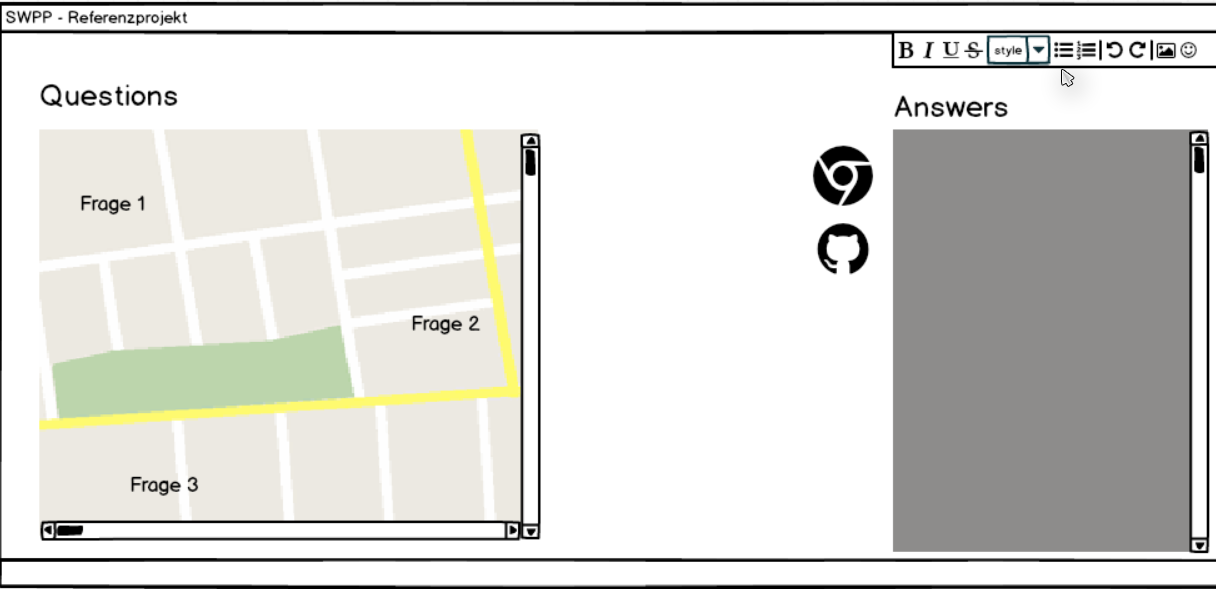
\includegraphics[width=1.8\linewidth]{screenshot002}
	\caption{}
	\label{fig:screenshot002}
\end{figure}




\subsection{Abnahmekriterien}


= Bezeichnung des letzten Schritts in der Systemauswahl
Erfolgt nach erfolgreich, abgeschlossenen Projektbetrieb.

Umfasst Hard- und Softwarekomponenten -> Berücksichtigung der Leistungsanforderungen

\textbf {natürlichsprachliches abstraktes Abnahmekriterium}

Ausgangssituation:
Mindestens 1 Nutzer ist in der App (virtuellen Welt) angemeldet

Ereignis:
Im Rahmen des Spielvorgangs der App kann der Nutzer seinen Charakter auswählen und sich auf die virtuelle Map begeben

erwartetes Ergebnis:
der Nutzer kann ohne Probleme auf der Map umhergehen und gestellte IT-Fragen beantworten in Form einer spielerischen Art


\textbf {formalisiert abstraktes Abnahmekriterium}

In Form einer Tabelle

Ablauf:


\begin{itemize}
	\item Nutzer hat die volle Kontrolle über seinen eigenen Charakter in der App bzw. Webseite
	
	\item Er kann seinen Charakter bearbeiten und PlugIns importieren, Mapskins und weitere Layoutänderung in der App vornehmen die       keinen Einfluss auf die Funktionalität haben
	
	\item Ihm wird ermöglicht Fehlerquellen beheben zu können 
	
	\item Bildschrimausgabe auf dem Screen des Nutzers
	
	\item Seine Ergebnisse der beantworteten Fragen können online
	 gespeichert oder lokal ausgedruckt werden -> Rangliste 
	 
\end{itemize}


\subsection{Pläne zur Evaluierung}

Wesentlich für seriöse und erfolgreiche (Selbst-)Evaluation sind vor allem …



\textbf {einsichtige Gründe und spürbare Folgen}
\begin{itemize}
	\item erweitern des Wissens in der Natur indem man zu Standorten auf der App läuft/geht und eine Frage beantwortet oder eine Frage erstellt
\end{itemize}




\textbf {ein positiver Ansatz}

\begin{itemize}
	\item einzigartig, aktuell, qualitativ hochwertig, Benutzerfreundlich
\end{itemize}




\textbf {relevante Fragestellungen und Kriterien}

\begin{itemize}
	\item möglichst viel Aufmerksamkeit der User bekommen
	\item Bekanntheitsgrad erhöhen
	\item Feedback von den Usern zur App bekommen
\end{itemize}




\textbf {wirksame Methoden und Instrumente}

\begin{itemize}
	\item App ist völlig Kostenlos
	\item leicht bedienbar
	\item für jede Altersklasse tauglich
\end{itemize}


\textbf {ein multiperspektivischer Ansatz}

Da unser Professor sich diese Applikation zunächst auf Fehler bzw. Macken analysiert und wir sie dann der Klasse vorstellen werden  wir uns wahrscheinlich die ein oder andere Idee noch einbauen oder einen Prototypen erstellen bevor wir es im Markt präsentieren.

\textbf {klare Verantwortlichkeiten und Entscheidungsstrukturen}


Verantwortlich für Projekt/App bzw. Webseite sind wir selbst. (Christopher Haider und Maximilian)
Entscheidungen werden nur durch Christopher Haider den Projektleiter zustande kommen.
Mehr Informationen zu den jeweiligen Themen finden Sie oben bei der Abbildung 1.6.


\textbf {machbare Pläne und gesicherte Rahmenbedingungen}

Qualifikationen: Beteiligte dieses Projektes besitzen spezielle Fachkenntnisse bzw. Qualifikationen

Zeit: Unser Plan ist es dieses Projekt bis Ende Schulschluss fertigzustellen.

Geldmittel: 


\subsection{Ergänzungen und zu klärende Punkte}

\chapter{Vorstellung des Produktes}
Vorstellung des fertigen Produktes anhand von Screenshots, Bildern, Erklärungen.

\chapter{Eingesetzte Technologien}
\begin{itemize}
	\item Kurzbeschreibung aller Technologien, die verwendet wurden.
	\item Technologien die aus dem Unterricht bekannt sind, nur nennen und deren  Einsatzzweck im Projekt beschreiben, nicht die Technologien selbst.
	\item Technologien die aus dem Unterricht nicht bekannt sind, im Detail beschreiben incl. deren Einsatz im Projekt
	\item Fokus aus eingesetzten Frameworks
\end{itemize}

\chapter{Problemanalyse}
\section{USE-Case-Analyse}
\begin{itemize}
	\item UseCases auf Basis von Benutzerzielen identifizieren: 
	\begin{itemize}
		\item Benutzer eines Systems identifizieren
		\item Benutzerziele identifizieren (Interviews)
		\item Use-Case-Liste pro Benutzer definieren
	\end{itemize}
	\item UseCases auf Basis von Ereignissen identifizieren: 
	\begin{itemize}
		\item Externes Event triggert einen Prozess
		\item zeitliches Event triggert einen Prozess (Zeitpunkt wird erreicht) 
		\item State-Event (Zustandsänderung im System triggert einen Prozess)
	\end{itemize}
	\item Werkzeuge:
	\begin{itemize}
		\item USE-Case-Beschreibungen (textuell, tabellarisch)
		\item USE-Case-Diagramm
		\item Aktivitätsdiagramm für den Use-Case (Interaktion zwischen Akteur und System abbilden)
		\item System-Sequenzdiagramm (Spezialfall eines Sequenzdiagramms: Nur 1 Akteur und 1 Objekt, das Objekt ist das komplette System, es geht um die Input/Output Requirements, die abzubilden sind)
	\end{itemize}
\end{itemize}

\section{Domain-Class-Modelling}
\begin{itemize}
	\item "Dinge" (Rollen, Einheiten, Geräte, Events etc.) identifizieren, um die es im Projekt geht
	\item ER-Modellierung oder Klassendiagramme
	\item Zustandsdiagramme (zur Darstellung des Lebenszyklus von Domain-Klassen darstellen)
\end{itemize}

\section{User-Interface-Design}
\begin{itemize}
	\item Mockups
	\item Wireframes
\end{itemize}


\chapter{Systementwurf}

\section{Architektur}

\subsection{Design der Komponenten}

Darstellung und Beschreibung der Systemarchitektur;

\begin{itemize}
	\item  statische Zerlegung des Systems in seine physischen Bestandteile (Komponenten, Komponentendiagramm)
	\item (textuelle) Beschreibung des dynamischen Zusammenwirkens aller Komponenten 
	\item (textuelle) Beschreibung der Strategie für die Architektur, d. h. wie die Architektur in Statik und Dynamik funktionieren soll.
	\item Verwendung von Referenzarchitekturen bzw. Architekturmustern (als Schablonen, z.B. MVC. Plugin, Pipes and Filters)
	\begin{itemize}
		\item MVC
		\item Schichten
		\item Pipes
		\item Request Broker
		\item Service-Oriented
	\end{itemize}
\end{itemize}

\subsection{Benutzerschnittstellen} 
\begin{itemize}
	\item Design des UIs
	\item Dialoge, Dialogsteuerung, Ergonomie, Gestaltung, Eingabeüberprüfungen
\end{itemize}

\subsection{Datenhaltunskonzept}
\begin{itemize}
	\item Design der Datenbank (ER-Modell)
	\item Design des Zugriffs auf diese Daten (Datenhaltungskonzept)
	\item Caching, Transaktionen
\end{itemize}

\subsection{Konzept für Ausnahmebehandlung}
\begin{itemize}
	\item Systemweite Festlegung, wie mit Exceptions umgegangen wird
	\item Exceptions sind primär aus den Bereichen UI, Persistenz, Workflow-Management
\end{itemize}

\subsection{Sicherheitskonzept}
Beschreibung aller sicherheitsrelevanten Designentscheidungen

\begin{itemize}
	\item Design der Security-Elemente
	\item Design von Safety-Elementen (Fehlertoleranz, Verfügbarkeit etc.)
\end{itemize}

\subsection{Design der Testumgebung}
\begin{itemize}
	\item wie wird getestet (Unit-Testing, Integrationstesting, Systemtests, Akzeptanztests)
	\item Testumgebung, Testprozess, Teststrategie, Testmethoden, Testfälle
\end{itemize}


\subsection{Desing der Ausführungsumgebung}
\begin{itemize}
	\item Deployment (DevOps)
	\item Betrieb (besonders Hoch- und Hertunerfahren der Anwendung)
\end{itemize}

\section{Detailentwurf}

Design jedes einzelnen USE-Cases

\begin{itemize}
	\item Design-Klassendiagramme vom Domain-Klassendiagramm ableiten (incl. detaillierter Darstellung und Verwendung von Vererbungshierarchichen, abstrakten Klassen, Interfaces)
	\item Sequenzdiagramme vom System-Sequenz-Diagramm ableiten
	\item Aktivitätsdiagramme
	\item Detaillierte Zustandsdiagramme für wichtige Klassen
\end{itemize}

Verwendung von CRC-Cards (Class, Responsibilities, Collaboration) für die Klassen
\begin{itemize}
	\item um Verantwortlichkeiten und Zusammenarbeit zwischen Klassen zu definieren und
	\item um auf den Entwurf der Geschäftslogik zu fokussieren
\end{itemize}

Design-Klassen für jeden einzelnen USE-Case können z.B. sein:

\begin{itemize}
	\item UI-Klassen
	\item Data-Access-Klassen
	\item Entity-Klassen (Domain-Klassen)
	\item Controller-Klassen
	\item Business-Logik-Klassen
	\item View-Klassen
\end{itemize}

Optimierung des Entwurfs (Modularisierung, Erweiterbarkeit, Lesbarkeit):

\begin{itemize}
	\item Kopplung optimieren
	\item Kohäsion optimieren
	\item SOLID
	\item Entwurfsmuster einsetzen
\end{itemize}

\chapter{Implementierung}
Detaillierte Beschreibung der Implementierung aller Teilkomponenten der Software entlang der zentralsten Use-Cases:

\begin{itemize}
	\item GUI-Implementierung
	\item Controllerlogik
	\item Geschäftslogik
	\item Datenbankzugriffe
\end{itemize}

Detaillierte Beschreibung der Teststrategie (Testdriven Development):

\begin{itemize}
	\item UNIT-Tests (Funktional)
	\item Integrationstests
\end{itemize}

Zu Codesequenzen:
\begin{itemize}
	\item kurze Codesequenzen direkt im Text (mit Zeilnnummern auf die man in der Beschreibung verweisen kann)
	\item lange Codesequenzen in den Anhang (mit Zeilennummer) und darauf verweisen (wie z.B. hier \cref{qj})
\end{itemize}

\chapter{Deployment}
\begin{itemize}
	\item Umsetzung der Ausführungsumgebung
	\item Deployment
	\item DevOps-Thema
\end{itemize}

\chapter{Tests}

\section{Systemtests} 
Systemtests aller implementierten Funktionalitäten lt. Pflichtenheft
\begin{itemize}
	\item Beschreibung der Teststrategie
	\item Testfall 1
	\item Testfall 2
	\item Tesfall 3
	\item …
\end{itemize}

\section{Akzeptanztests}

\chapter{Projektevaluation}
siehe Projektmanagement-Unterricht

\chapter{Benutzerhandbuch} 
falls im Projekt gefordert

\chapter{Betriebswirtschaftlicher Kontext}
BW-Teil

\chapter{Zusammenfassung}
\begin{itemize}
	\item Etwas längere Form des Abstracts
	\item Detaillierte Beschreibung des Outputs der Arbeit
\end{itemize}
\chapter{Beispielkapitel}
\section{Beispiele zitieren}

Das ist ein Zitat mit Klammern,
\citep{resnick_distributed_1996}, das ein Zitat ohne Klammern:
\cite{harel_situating_1991}. Hier das selbe Zitat mit einer Seitenangabe und Klammern \citep[S. 23]{resnick_distributed_1996}.

Wird ein Absatz aus einer Quelle sinngemäß übernommen (nicht wörtlich), dann kann nach dem Absatz das entsprechende Zitat in Klammern angeführt werden. \citep[S. 33]{anastopoulou_constructionism_2012}

Wenn ein Zitat im Text angegeben wird, wie z.B. so \cite{beer_rudolf_aspekte_2011}, können die Klammern weggelassen werden.

Der folgende Absatz zeigt ein Blockzitat (wörtlich übernommene Textpassage aus einer Quelle):

\blockcquote[S. 21]{ackermann_piagets_2001}{
Dr. Heinrich Faust ist ein angesehener Wissenschaftler und Akademiker, der trotz seiner wissenschaftlichen Studien und einer guten Bildung seinen Wissensdurst nicht stillen kann. Eines Nachts sitzt er in seinem Studierzimmer und grübelt über den Sinn des Lebens nach, findet jedoch keine Antworten.
Daraufhin wendet er sich der Geisterwelt zu. Er beschwört einen Erdgeist, versucht sich den Geistern gleich zu stellen, was ihm jedoch nicht gelingt. Von Ohnmacht getrieben will er sich das Leben nehmen. Sein Selbstmordversuch wird jedoch von Glockenläuten zum Ostertag und seinen Kindheitserinnerungen gestört.
}

Hier wird ein wörtliches Zitat inline angegeben: \blockcquote{gohlich_lernen:_2007}{Das ist ein kleines direktes Zitat.}, und danach geht es gleich wieder direkt weiter. Ob ein wörtliches Zitat inline oder als eigener Block angezeigt wird, entscheidet Latex auf Basis der Länge.

%So kann man den Author umdefinieren, der für den Seiteninhalt
%verantwortlich ist
\def \currentAuthor {Harald Sohm}

\subsection{Beispiele Abbildungen}
Auf diese Weise kann man zum Beispiel in Latex auf die \cref{fig:ArduExample} verweisen. Die Kennung für den Verweis vergibt
man selbst mit dem "`label"' Kommando bei der Abbildung.

Jede Abbildung muss nicht nur mindestens einen Verweis im Text haben. Es wird außerdem eine Bildunterschrift verlangt. Für diese ist festgesetzt, dass die Abbildungsunterschrift alleine ausreichend sein muss, um zu verstehen, was am Bild zu erkennen ist. 

Der nächste wichtige Punkt sind die Quellenangaben bei Abbildungen. Der Author muss zu jeder Abbildung die notwendigen Rechte haben und idealer Weise gibt man diese bei der Abbildung mit an. In \cref{fig:ArduExample} auf Seite \pageref{fig:ArduExample} sieht man das.

Es ist wichtig zu verstehen, dass Latex die Positionierung von Abbildungen übernimmt. Man definiert die Abbildung über begin-figure dort, wo man die Abbildung in etwa haben  möchte, den Rest übernimmt Latex

\begin{figure}[t]
\centering
%\includegraphics[width=0.7\linewidth]{figures/Arduino_board.png}
\copyrightbox[r]{\includegraphics[width=0.8\linewidth]{figures/Arduino_Example.jpg}}{\textcopyright\
Stefan Stolz (CC BY-SA 3.0)}
\caption[Arduino mit Lichtsensor und Lichterkette]{Hintergrund: Arduino Board;
Vordergrund: eine Lichterreihe und ein Lichtsensor (Fotowiderstand); In diesem
Beispiel wird die Lichterreiche je nach Helligkeit des Umgebungslichtes
gesteuert. Durch leichte Modifikationen kann man damit eine Lichtschranke oder
auch eine Helligkeitssteuerung für das Smartphone simulieren.}
\label{fig:ArduExample}
\end{figure}

\subsubsection{Beispiele Tabellen}

\cref{tbl:shiftReg} ist ein Beispiel für eine aufwändigere Tabelle mit einer
Abbildung und Überschrift.

\begin{table}
     \begin{center}
     \begin{tabularx}{\textwidth}{ cX  } 
      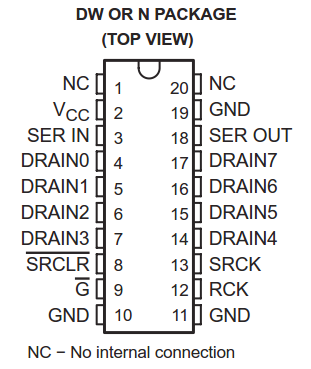
\includegraphics[width=0.3\textwidth]{figures/shift_reg.png}  & 
      {\begin{tabularx}{\cellwidth}{ lX  }      
      $V_{cc}$ & Positive supply voltage\\
      GND & Ground \\
      SER IN & Daten Pin \\
      SRCK & Clock Pin \\
      RCK & Latch Pin \\
      $\overline{SRCLR}$ & Wenn \textbf{shift-register clear} LOW ist, werden die input Register gelöscht\\
      $\overline{G}$ & Wenn \textbf{output enable} HIGH ist, werden die Daten im Output Buffer LOW gehalten
      \end{tabularx}   }
      \end{tabularx}
      \caption{Aufwändige Tabelle mit Abbildung und Caption}
      \label{tbl:shiftReg}
      \end{center}
\end{table}

Tabellen sind in Latex sehr kompliziert zu erzeugen. Alternativ kann man die Tabellen auch in einem anderen Programm gestalten und als Bild wieder einfügen. Dieses Bild kann dann innerhalb von begin-Table verwendet werden.

\section{Beispiele Listen}
Im Folgenden wird eine Liste gezeigt:
\begin{itemize}
  \item Ich weiß, dass viele Geräte des täglichen Lebens durch Computer
  gesteuert werden und kann für mich relevante nennen und nutzen.
  \begin{enumerate}
  	\item Und jetzt eine Numerierung
  	\item Und jetzt eine Numerierung
  \end{enumerate}
  \item Ich kann wichtige Bestandteile eines Computersystems (Eingabe-,
  Ausgabegeräte und Zentraleinheit) benennen, kann ihre Funktionen beschreiben
  und diese bedienen.
\end{itemize}

Und jetzt eine Numerierung:

\begin{enumerate}
	\item Aufzählungspunkt
	\begin{enumerate}
		\item Unteraufzählung
		\item Unteraufzählung
		\begin{itemize}
			\item Und jetzt noch eine Ebene ohne Aufzählung
			\item Und jetzt noch eine Ebene ohne Aufzählung
		\end{itemize}
	\end{enumerate}
	\item Aufzählungspunkt
	\item Aufzählungspunkt
	\item Aufzählungspunkt
	\item Aufzählungspunkt
\end{enumerate}

\section{Beispiel Codesequenz}
In \cref{code:qj} sieht man ein Quick-Sort-Listing in der Programmiersprache JAVA. Das Listings-Paket übernimmt die Formatierung von Codebausteinen und kann in der Präambel nach Belieben auf eine andere Sprache konfiguriert werden.

\def \currentAuthor {Author2}

\subsection{Quicksort in JAVA}
\begin{lstlisting}[language=Java, caption=QuickSort in Java, label=code:qj]
public class QuickSort {
public static void main(String[] args) {
int[] x = { 9, 2, 4, 7, 3, 7, 10 };
System.out.println(Arrays.toString(x));

int low = 0;
int high = x.length - 1;

quickSort(x, low, high);
System.out.println(Arrays.toString(x));
}

public static void quickSort(int[] arr, int low, int high) {
if (arr == null || arr.length == 0)
return;

if (low >= high)
return;

// pick the pivot
int middle = low + (high - low) / 2;
int pivot = arr[middle];

// make left < pivot and right > pivot
int i = low, j = high;
while (i <= j) {
while (arr[i] < pivot) {
i++;
}

while (arr[j] > pivot) {
j--;
}

if (i <= j) {
int temp = arr[i];
arr[i] = arr[j];
arr[j] = temp;
i++;
j--;
}
}

// recursively sort two sub parts
if (low < j)
quickSort(arr, low, j);

if (high > i)
quickSort(arr, i, high);
}
}
\end{lstlisting}

\section{Beispieltext}

\Blindtext

\listoffigures

\listoftables

\lstlistoflistings

\bibliographystyle{dinat}
%\bibliographystyle{plainurl}
\bibliography{Literatur_Verzeichnis} 

\appendix
\chapter{Anhang-Kapitel}
\section{Anhang-Section}
Testtext

\end{document}